\subsection{Seeds Data}

This data set has been used in the work of \cite{charytanowicz2010complete}. The data comprises information on different features of wheat kernels. There are seven species with a total of about 20 varieties of which three can be found in the data: Kama, Rosa and Canadian wheat. There is a total of 210 data points, evenly split between the varieties. The kernels for which data was collected were selected randomly. They were then examined through X-ray imaging. A software called \textit{GRAINS} for this specific application \cite{strumillo1999computer} was used to extract the features for each observation:
\begin{multicols}{2}
\begin{itemize}
\item area $A$
\item perimeter $P$
\item compactness $C = 4 \pi A/P^{2}$
\item length (along groove)
\item width
\item asymmetry coefficient
\item length of kernel groove
\item label
\end{itemize}
\end{multicols}

\begin{figure}[h]
\caption{Seeds pairplot WIP}
%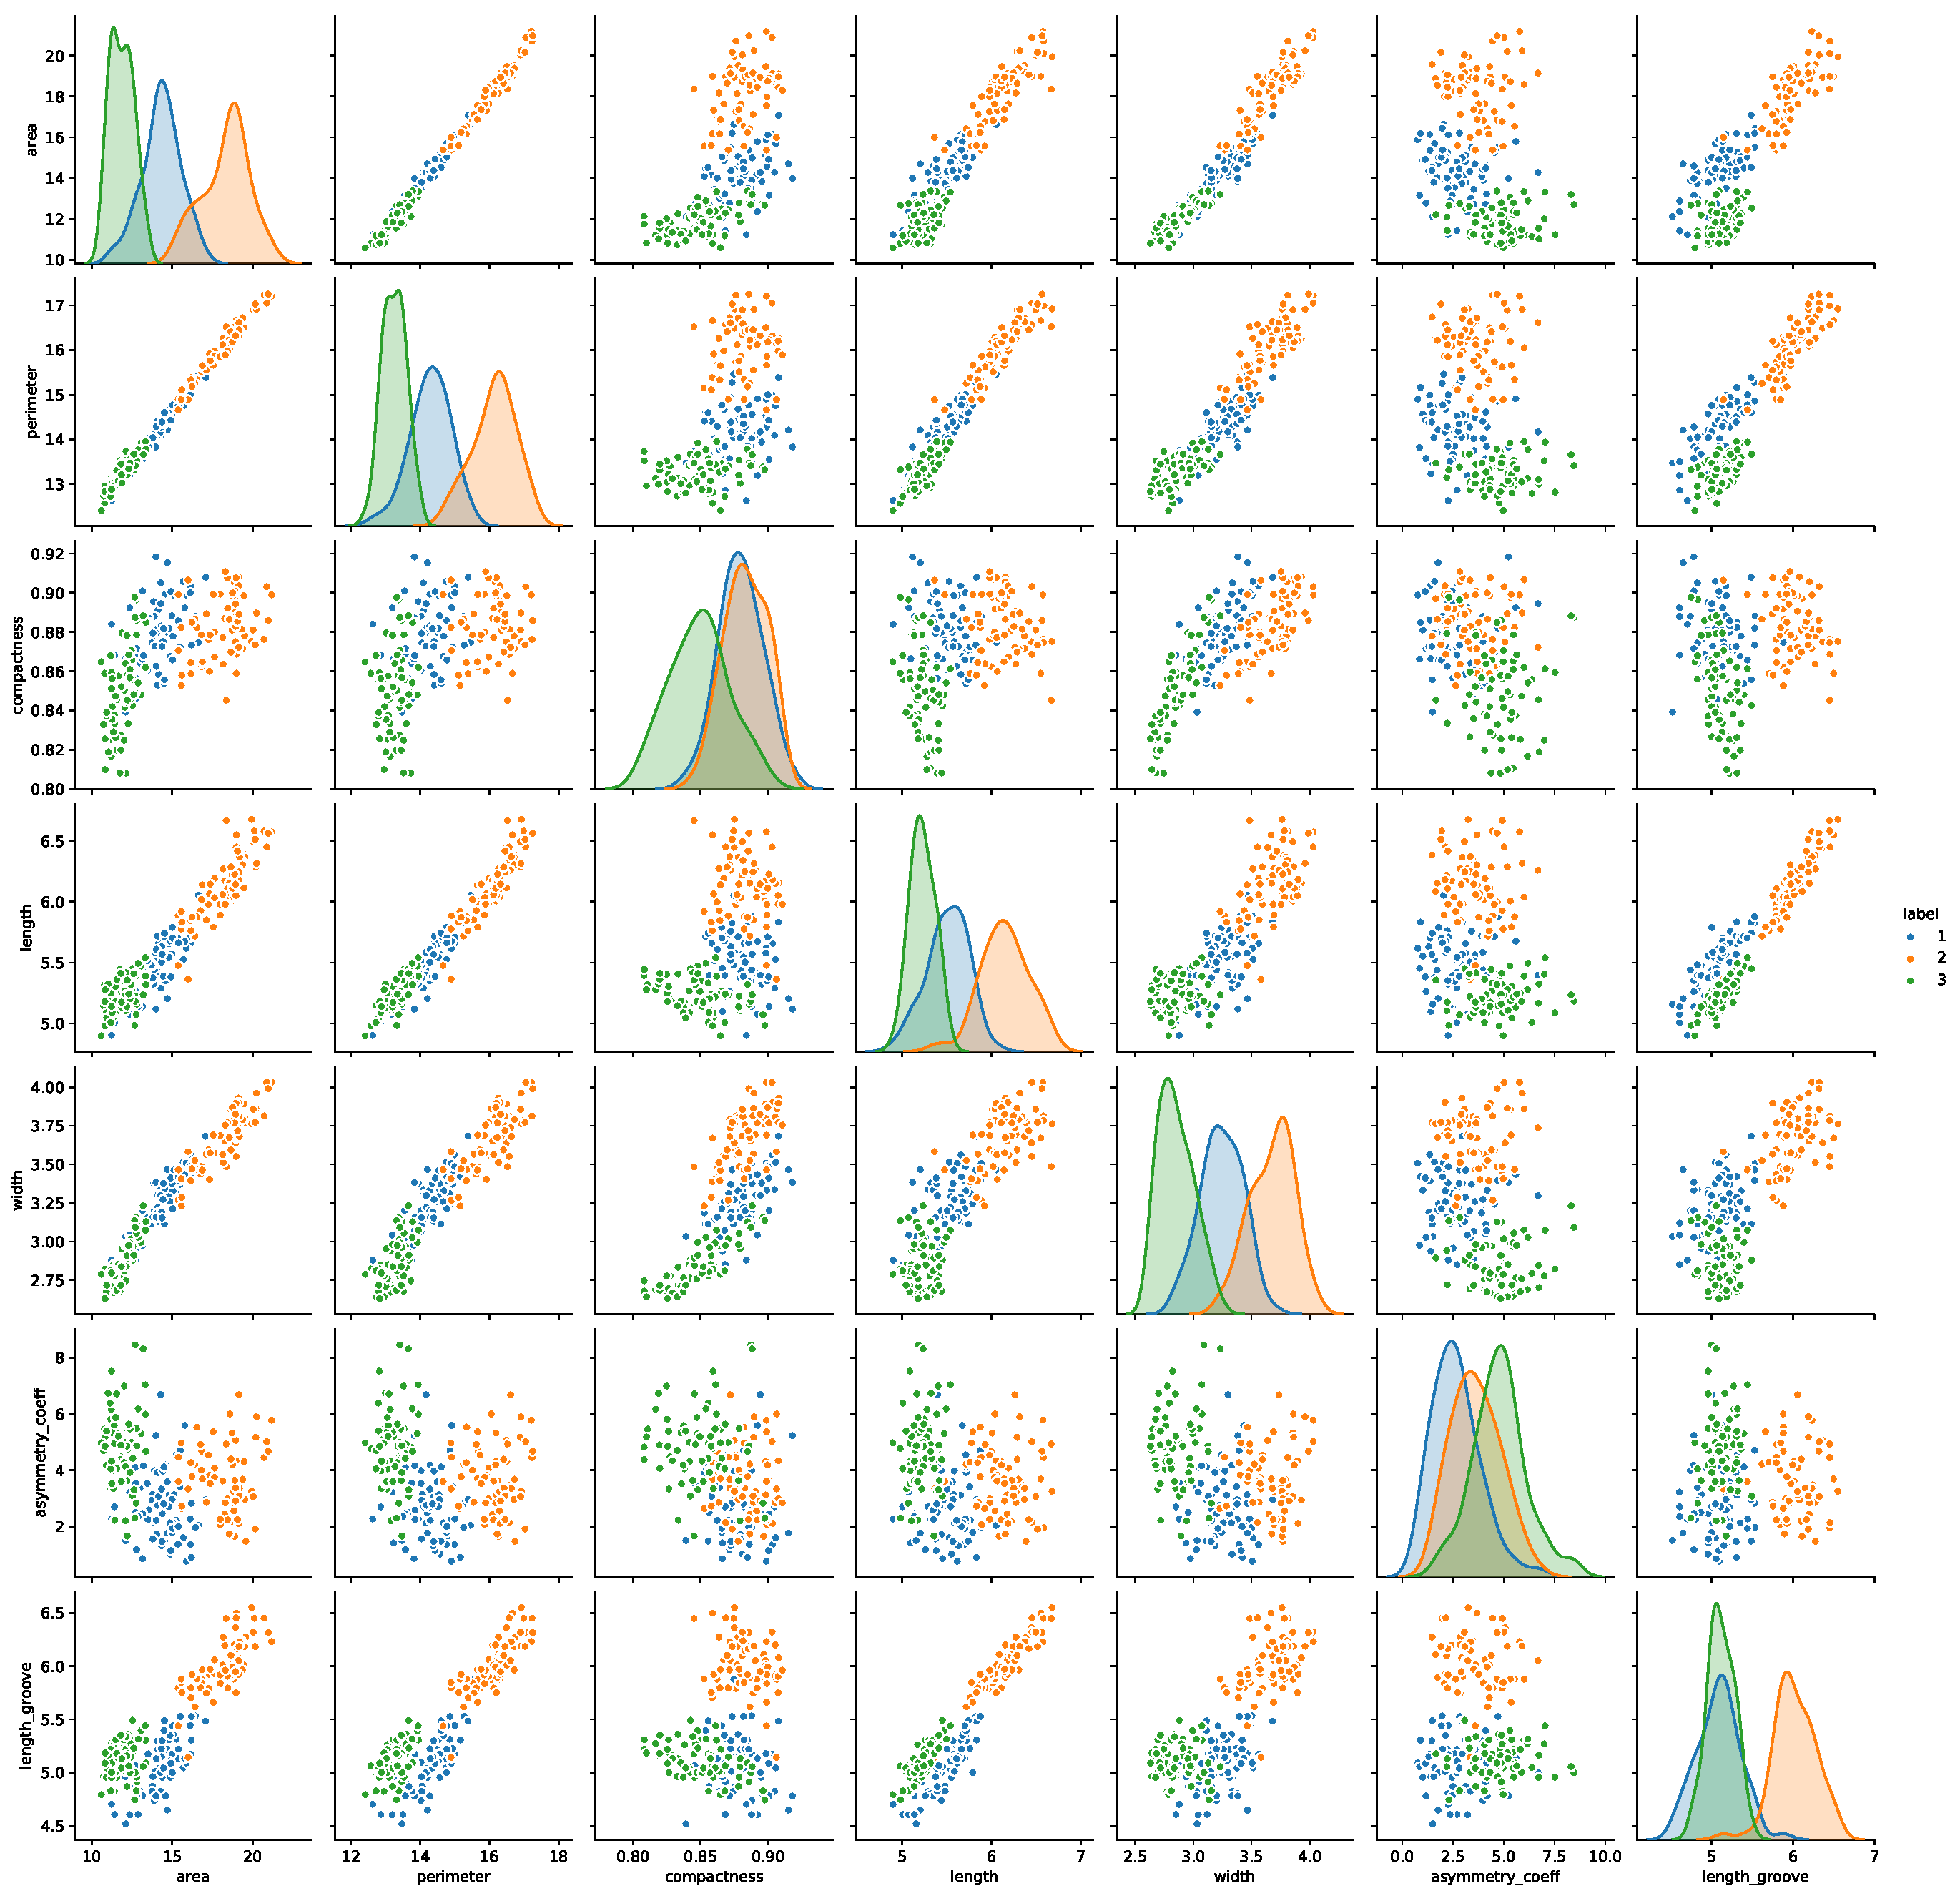
\includepdf[pages=-,scale=.4]{images/seeds_pairplot.pdf}
\begin{center}
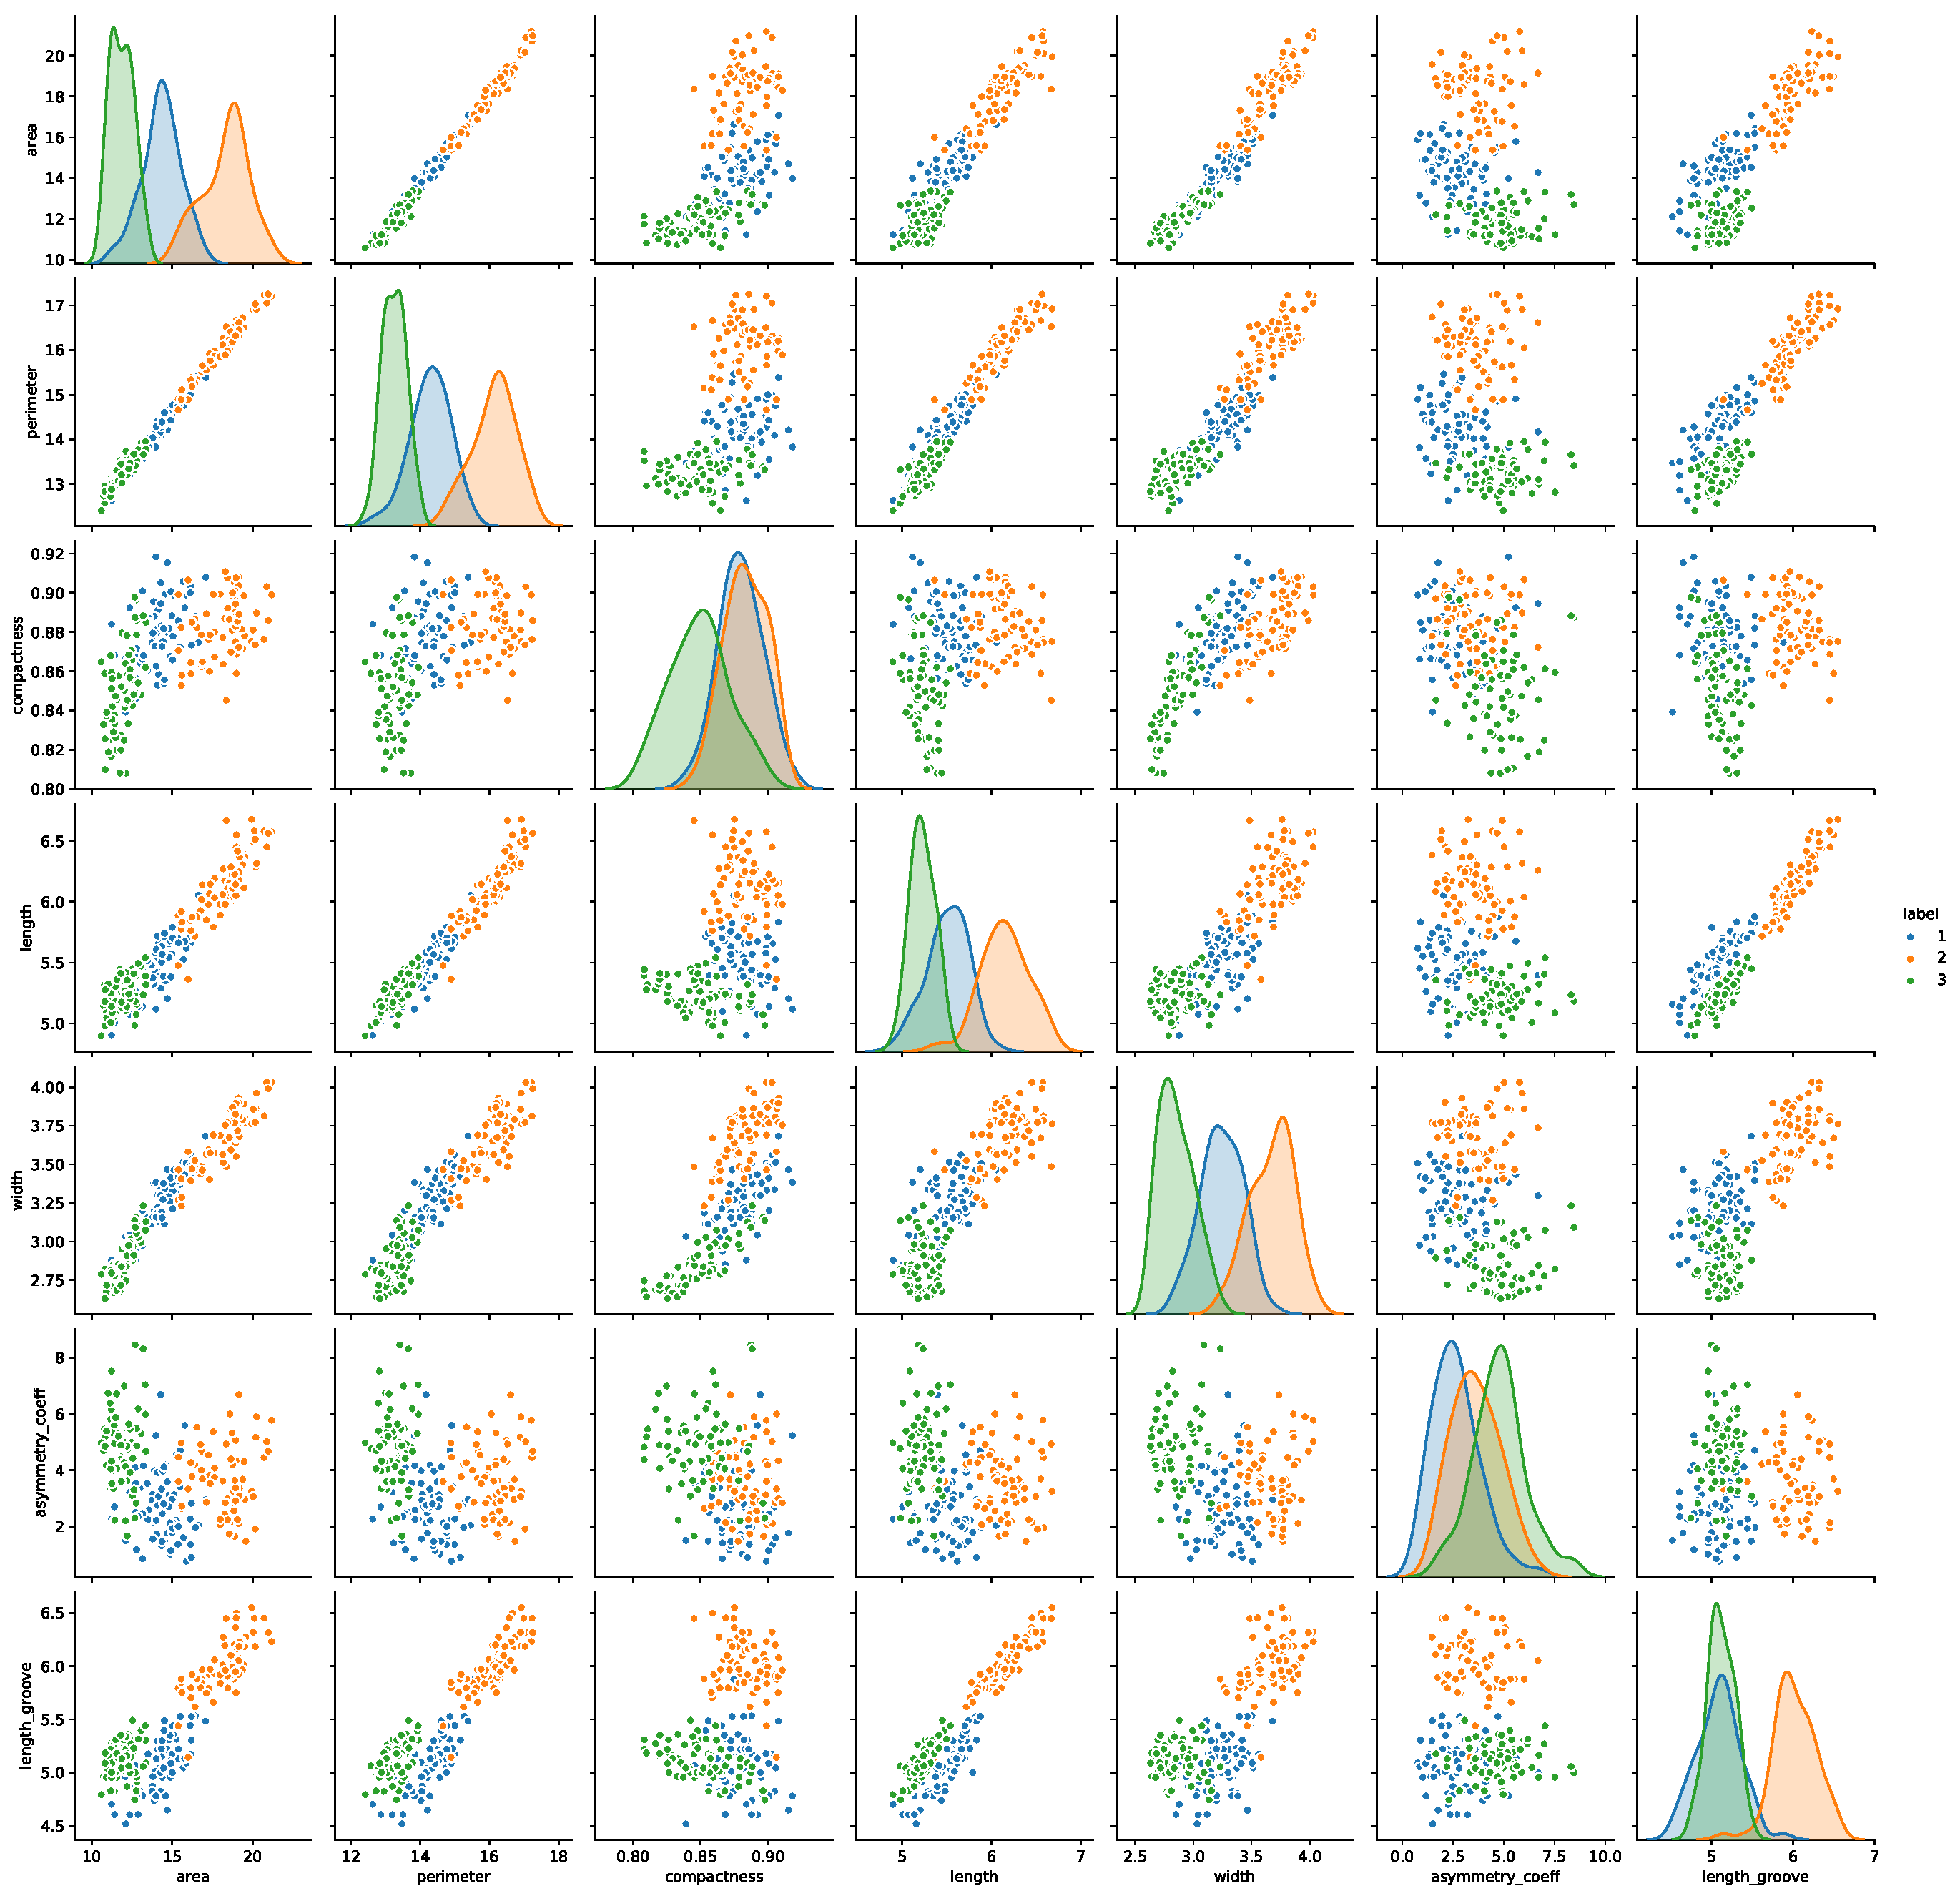
\includegraphics[width=0.75\textwidth]{images/seeds_pairplot.pdf}
\end{center}
\label{img:seeds_pairplot}
\end{figure}

A few things can be noted here: compactness is linearly dependent on two other features in the data set, calling into question what value this information can bring to a clustering method. Furthermore the area is not computed from other measurements, but is highly correlated with width and length and the perimeter. These relationships among others can be seen in figure \ref{img:seeds_pairplot}. Note that these plots have been colored according to their labels. Density plots on the diagonal already show distinct characteristics for the different varieties of kernels for certain features. For the clustering step of course the labels are removed from the data (this data set was included despite not being the typical application of clustering because it can serve as a sort of "control" for the clustering methods when looking at evaluation and conclusions).



